\section{結果のクイック描画:net2g} \label{sec:quicklook}
%####################################################################################

本節では、\verb|netcdf2grads|の使用方法を説明する。
プログラム\verb|netcdf2grads| (略して \verb|net2g|)は、プロセス毎に分割された{\netcdf}ファイル(\verb|history.**.nc|
\footnote{「gpview」がインストールされている場合には、「gpview」でも作図することができる。
このツールは historyデータを変換することなく直接作図することができるため、
素早く結果を確認した場合には適している。
}
)
を{\grads}形式の単一のバイナリファイルに結合する。
この変換した{\grads}バイナリデータを使って、シミュレーションの結果を確認する。


\subsubsection{{\grads}バイナリに変換}
%-----------------------------------------------------------------------------------
プロセスごとに分割された{\netcdf}形式のヒストリファイルから{\grads}バイナリに変換するために、\verb|net2g|を使用する。
ここでは最低限の手順のみを説明することにする。
詳細な使用方法は\ref{sec:net2g}節を参照されたい。

まず、\verb|net2g|ディレクトリに移動する。
\begin{verbatim}
 $ cd ${Tutorial_DIR}/real/experiment/net2g
 $ ls
    Makefile
    net2g -> ../../../../../util/netcdf2grads_h/net2g
    net2g.2D.d01.conf
    net2g.3D.d01.conf
\end{verbatim}
このディレクリの中には設定ファイルとバイナリファイルがある。
バイナリファイルは、\ref{sec:compile_net2g}節でコンパイルした実行ファイルにリンクされている。
ここでは例として、2次元変数のMSLP、PRECを{\grads}形式に変換する手順を示す。
また、3次元変数の 東西風(Umet)、南北風(Vmet)を 850 hPa 面、500hPa 面、200 hPa 面で抽出して、
{\grads}形式に変換する手順も説明する。
2次元変数と3次元変数のための設定ファイルはそれぞれ、
\verb|net2g.2D.d01.conf| と \verb|net2g.3D.d01.conf| である。

\verb|net2g|を実行する時のプロセス数は、
シミュレーションの実行時に用いたプロセス数の約数である必要がある。
ここでは、4プロセスを使用する。
net2g は2次元変数と3次元変数を同時に変換できないために、
以下のように別々に実行する。
\begin{verbatim}
 $ mpirun -n 4 ./net2g net2g.2D.d01.conf
 $ mpirun -n 4 ./net2g net2g.3D.d01.conf
\end{verbatim}
エラーメッセージがなく、下記のメッセージだけが標準出力へ表示されていれば、
変換は正常に完了している。\\

\noindent {\gt
\fbox{
\begin{tabularx}{150mm}{l}
\verb|+++ MPI COMM: Corrective Finalize| \\
\end{tabularx}
}}\\

成功すれば、下記のファイルが作成される。
\verb|**.ctl|は {\scalerm} のXY格子系に対するctlファイル、
\verb|**lccr.ctl|は緯度経度座標系で結果を作図するためのctlファイルである。

\begin{verbatim}
  MSLP_d01z-2d.ctl
  MSLP_d01z-2d.grd
  MSLP_d01z-2d_lccr.ctl
  PREC_d01z-2d.ctl
  PREC_d01z-2d.grd
  PREC_d01z-2d_lccr.ctl
  PRES_d01z-3d.ctl
  PRES_d01z-3d.grd
  PRES_d01z-3d_lccr.ctl
  Umet_d01z-3d.ctl
  Umet_d01z-3d.grd
  Umet_d01z-3d_lccr.ctl
  Vmet_d01z-3d.ctl
  Vmet_d01z-3d.grd
  Vmet_d01z-3d_lccr.ctl
\end{verbatim}




\subsubsection{計算結果の確認}
%-----------------------------------------------------------------------------------

%\verb|${Tutorial_DIR}/real/data|ディレクトリに用意してあるので、
%サンプルとして利用してほしい。\footnote{今後、緯度経度座標で描画するためのctlファイルを出力できるようにする予定。}
%\begin{verbatim}
% $ cp ../../data/*_lcc.ctl ./
% $ ls
%    MSLP_d01z-2d_lcc.ctl
%    PREC_d01z-2d_lcc.ctl
%    U_d01z-3d_lcc.ctl
%    V_d01z-3d_lcc.ctl
%\end{verbatim}

\grads スクリプト\verb|checkfig_real.gs|を用いて、計算結果を確認する。
\begin{verbatim}
 $ cp ../../data/checkfig_real.gs ./
 $ grads -blc checkfig_real.gs
\end{verbatim}
変換が正常に終了すれば、下記のファイルが作成される。
なお、\grads のバージョンによって文法が異なるので、警告が出る場合はスクリプトを適宜変更されたい。
\begin{verbatim}
  real_mslp.png
  real_prec.png
  real_wind.png
\end{verbatim}
計算が成功していれば、
図\ref{fig:real_mslp}, \ref{fig:real_prec}, \ref{fig:real_wind}と同じ図が得られる。


\begin{figure}[h]
\begin{center}
  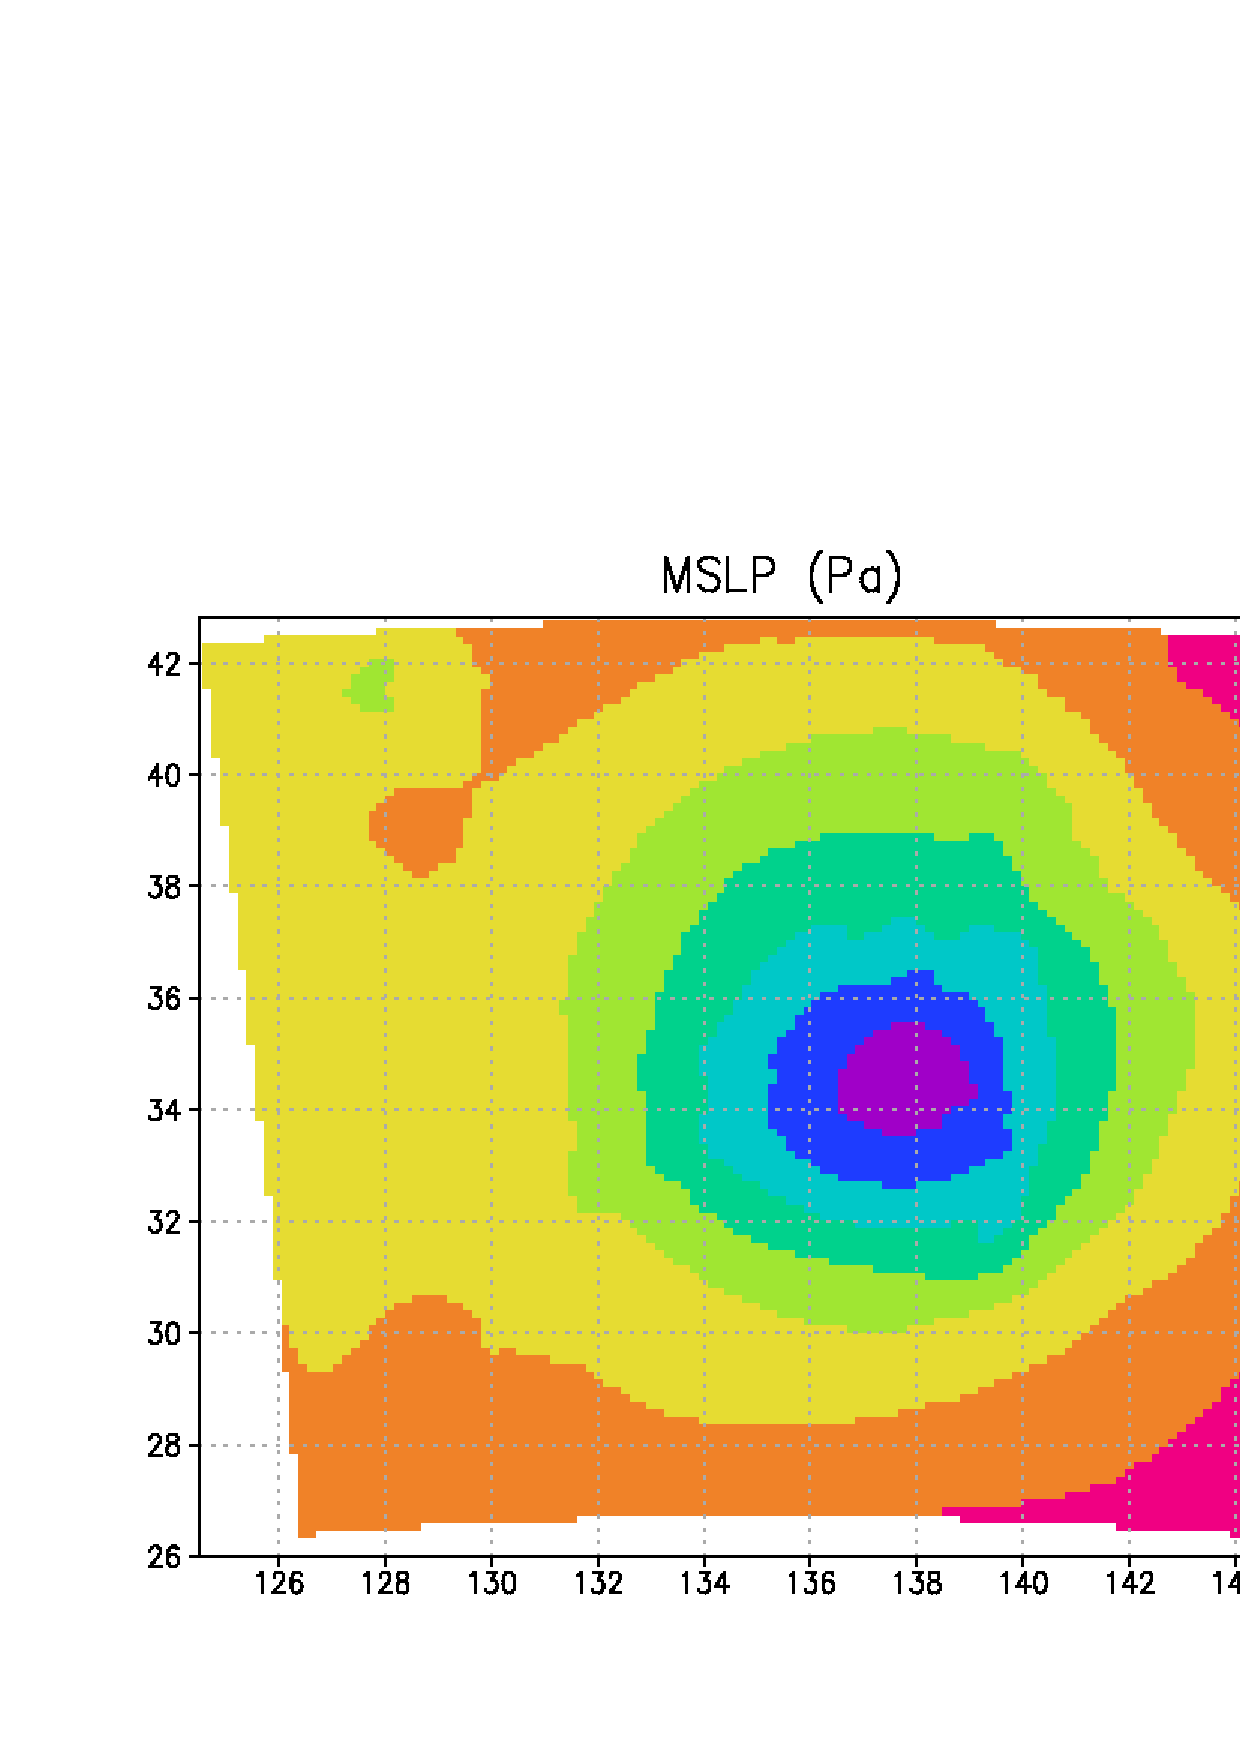
\includegraphics[width=0.55\hsize]{./../../figure/real_mslp.pdf}\\
  \caption{計算開始から6時間後の海面更正気圧}
  \label{fig:real_mslp}
\end{center}
\begin{center}
  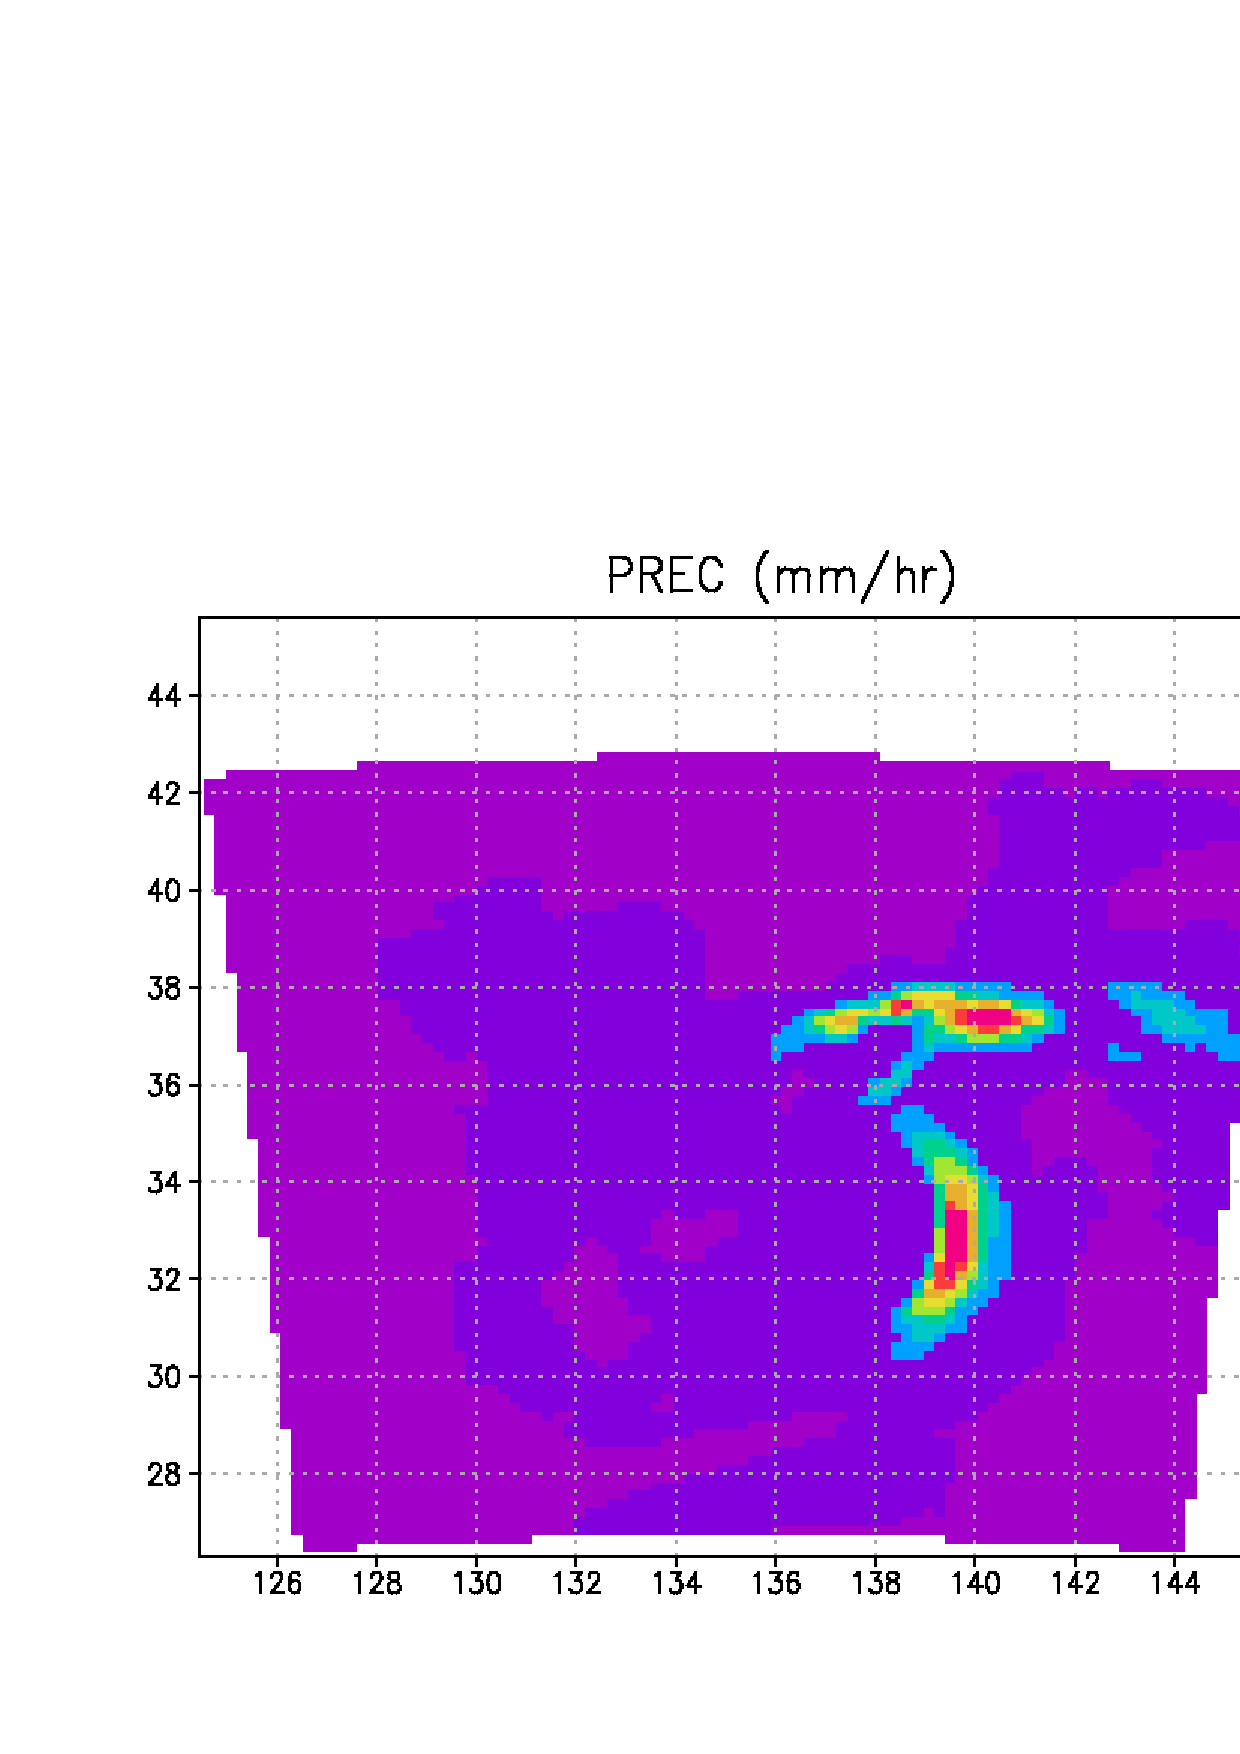
\includegraphics[width=0.55\hsize]{./../../figure/real_prec.pdf}\\
  \caption{計算開始から6時間後の降水フラックス}
  \label{fig:real_prec}
\end{center}
\begin{center}
  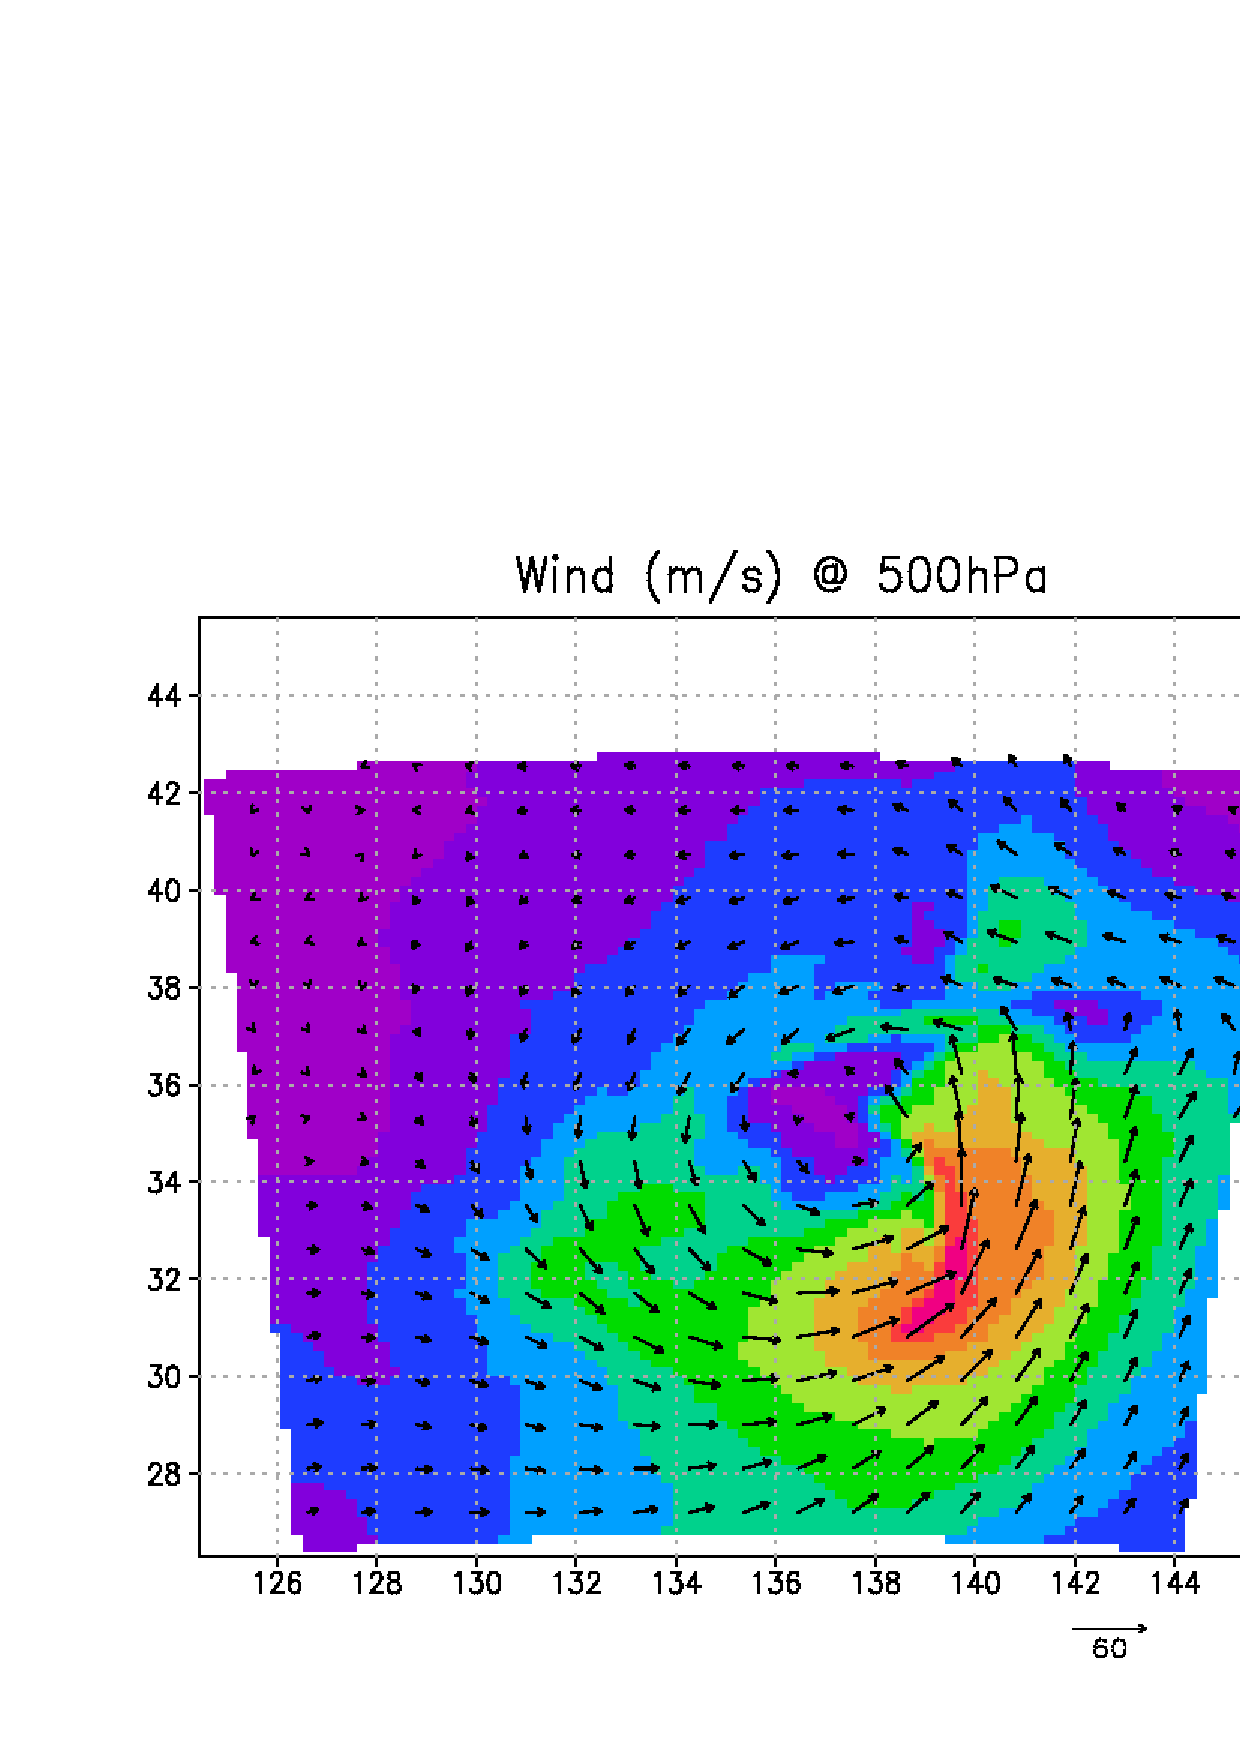
\includegraphics[width=0.55\hsize]{./../../figure/real_wind.pdf}\\
  \caption{計算開始から6時間後の850hPaの風速(色は絶対値、ベクトルは向き)}
  \label{fig:real_wind}
\end{center}
\end{figure}
